\subsection{Metric Spaces and Euclidean Topology}\label{subsec:metric-spaces-and-euclidean-topology}

% **Role:** abstract structure behind limits and continuity.
%
% Metrics, open/closed sets, neighborhoods, closure, interior, boundary, limit points, relative topology.


Metric topology studies sets through balls: openness, closure, and limit points come from distance. Euclidean estimates rely on norms, Cauchy--Schwarz, and the triangle inequality.

\begin{definition} \label{def:metric-space} \hlt{Metric Space}\\
A \hlt{metric space} is a set $X$ equipped with a function $d:X\times X\to\R$ such that, for all $p,q,r\in X$,
\begin{enumerate}[label=\roman*.]
\setlength{\itemsep}{0pt}
\item $d(p,q)>0$ if $p\neq q$, and $d(p,p)=0$;
\item $d(p,q)=d(q,p)$;
\item $d(p,q)\leq d(p,r)+d(r,q)$.
\end{enumerate}
The function $d$ is called a \hlt{distance function} or \hlt{metric}.
\end{definition}

\begin{perspective} \label{per:epsilon-closeness-to-metric-language} \hlt{$\varepsilon$-Closeness Becomes Metric Language}\\
On $\R$, $\varepsilon$-close means $\abs{x-y}<\varepsilon$, i.e. $d(x,y)<\varepsilon$ with $d(x,y)=\abs{x-y}$; may be abstracted to metric balls.\\
\hlt{Key Insight}: Absolute value is distance on $\R$.
\end{perspective}

\begin{example} \label{ex:euclidean-metric-and-subspaces} \hlt{Euclidean Metric and Subspaces}\\
The Euclidean space $\R^k$ is a metric space with $d(\mathbf{x},\mathbf{y})\defeq\norm{\mathbf{x}-\mathbf{y}}_2,\qquad \mathbf{x},\mathbf{y}\in\R^k$.\\
Every subset $Y$ of a metric space $X$ is a metric space by restricting the same distance function to points of $Y$.
\end{example}

\begin{example} \label{ex:discrete-metric} \hlt{Discrete Metric}\\
On any set $X$, define $d(x,y)=
\begin{cases}
0, & x=y,\\
1, & x\neq y.
\end{cases}$.\\
This is the \hlt{discrete metric}: distinct points are all distance $1$ apart.
\end{example}

\begin{example} \label{ex:hamming-distance} \hlt{Hamming Distance}\\
For $x,y\in\{0,1\}^n$, define $h(x,y)\defeq\abs{\{i:x_i\neq y_i\}}$. Then $h$ is a metric.
\begin{proof}
$h\geq0$, $h(x,y)=h(y,x)$, and $h(x,y)=0\Longleftrightarrow x_i=y_i\ \forall i\Longleftrightarrow x=y$.\\
For $x,y,z\in\{0,1\}^n$, $\{i:x_i\neq y_i\}\subseteq\{i:x_i\neq z_i\}\cup\{i:z_i\neq y_i\}$, so $h(x,y)\leq h(x,z)+h(z,y)$.\\
\hlt{Structural Commentary}: Hamming distance counts coordinate disagreements.\\
\hlt{Key Insight}: Each disagreement between $x$ and $y$ must be paid for through $z$ in at least one leg.
\end{proof}
\end{example}

\begin{example} \label{ex:coordinate-norm-metrics-rk} \hlt{Coordinate Norm Metrics on $\R^k$}\\
By Proposition \ref{prop:coordinate-norms-on-fn} and Theorem \ref{thm:cauchy-schwarz-inequality}, $d_1(\mathbf{x},\mathbf{y})\defeq\norm{\mathbf{x}-\mathbf{y}}_1$; $d_2(\mathbf{x},\mathbf{y})\defeq\norm{\mathbf{x}-\mathbf{y}}_2$; $d_\infty(\mathbf{x},\mathbf{y})\defeq\norm{\mathbf{x}-\mathbf{y}}_\infty$ are metrics on $\R^k$, and $\forall \mathbf{x},\mathbf{y}\in\R^k$, $d_\infty(\mathbf{x},\mathbf{y})\leq d_2(\mathbf{x},\mathbf{y})\leq d_1(\mathbf{x},\mathbf{y})\leq \sqrt{k}\,d_2(\mathbf{x},\mathbf{y})$; $d_2(\mathbf{x},\mathbf{y})\leq \sqrt{k}\,d_\infty(\mathbf{x},\mathbf{y})$.\\
Hence $d_1,d_2,d_\infty$ have the same convergent sequences.
\end{example}

\begin{theorem} \label{thm:holder-minkowski-sequence-spaces} \hlt{H\"older and Minkowski for Sequence Spaces}\\
Let $\mathbb{F}\in\{\R,\C\}$.
\begin{enumerate}[label=(\roman*)]
\setlength{\itemsep}{0pt}
\item If $p,q>1$ and $p^{-1}+q^{-1}=1$, then $\mathbf{x}\in\ell^p(\mathbb{F})$, $\mathbf{y}\in\ell^q(\mathbb{F})$ imply $\sum_{n\geq1}\abs{x_ny_n}\leq\norm{\mathbf{x}}_p\norm{\mathbf{y}}_q$.
\item If $1\leq p<\infty$ and $\mathbf{x},\mathbf{y}\in\ell^p(\mathbb{F})$, then $\mathbf{x}+\mathbf{y}\in\ell^p(\mathbb{F})$ and $\norm{\mathbf{x}+\mathbf{y}}_p\leq\norm{\mathbf{x}}_p+\norm{\mathbf{y}}_p$.
\end{enumerate}
\begin{proof}
\begin{enumerate}[label=(\roman*)]
\setlength{\itemsep}{0pt}
\item If $\norm{\mathbf{x}}_p\norm{\mathbf{y}}_q=0$, the claim is immediate.\\
Otherwise set $X\defeq\norm{\mathbf{x}}_p$, $Y\defeq\norm{\mathbf{y}}_q$, $u_n\defeq\abs{x_n}/X$, and $v_n\defeq\abs{y_n}/Y$. Young's inequality gives $u_nv_n\leq u_n^p/p+v_n^q/q$; summing over $1\leq n\leq N$ and letting $N\to\infty$ gives $\sum_{n\geq1}\abs{x_ny_n}\leq XY$.
\item For $p=1$, apply $\abs{x_n+y_n}\leq\abs{x_n}+\abs{y_n}$ and sum. For $p>1$, put $s_N\defeq(\sum_{n=1}^{N}\abs{x_n+y_n}^p)^{1/p}$. If $s_N=0$, the bound is trivial; if $s_N>0$, then $\sum_{n=1}^{N}\abs{x_n+y_n}^{p}\leq\sum_{n=1}^{N}(\abs{x_n}+\abs{y_n})\abs{x_n+y_n}^{p-1}\leq(\norm{\mathbf{x}}_p+\norm{\mathbf{y}}_p)s_N^{p-1}$ by (i), so $s_N\leq\norm{\mathbf{x}}_p+\norm{\mathbf{y}}_p$. Let $N\to\infty$.
\end{enumerate}
\hlt{Structural Commentary}: H\"older controls products; Minkowski controls sums.\\
\hlt{Key Insight}: The metric property of $\ell^p$ is exactly Minkowski's inequality.
\end{proof}
\end{theorem}

\begin{example} \label{ex:function-and-sequence-metric-spaces} \hlt{Function and Sequence Metric Spaces}\\
Let $\mathbb{F}\in\{\R,\C\}$.
\begin{enumerate}[label=(\roman*)]
\setlength{\itemsep}{0pt}
\item On $C_{\mathbb{F}}[a,b]$, $d_\infty(f,g)\defeq\sup_{t\in[a,b]}\abs{f(t)-g(t)}$ and $d_1(f,g)\defeq\int_a^b\abs{f(t)-g(t)}\,dt$ are metrics.\\
Definiteness of $d_1$ uses continuity.
\item On $\ell^\infty(\mathbb{F})$, $d_\infty(\mathbf{x},\mathbf{y})\defeq\sup_{n\geq1}\abs{x_n-y_n}$ is a metric.
\item For $1\leq p<\infty$, $d_p(\mathbf{x},\mathbf{y})\defeq\norm{\mathbf{x}-\mathbf{y}}_p=(\sum_{n\geq1}\abs{x_n-y_n}^p)^{1/p}$ is a metric on $\ell^p(\mathbb{F})$ by Theorem \ref{thm:holder-minkowski-sequence-spaces}.
\end{enumerate}
\hlt{Structural Commentary}: Norm estimates produce metrics on function and sequence spaces.\\
\hlt{Key Insight}: Infinite-dimensional examples require estimates, not just coordinate formulas.
\end{example}

\begin{definition} \label{def:euclidean-intervals-cells-balls-convex} \hlt{Euclidean Intervals, Cells, Balls, and Convexity}
\begin{enumerate}[label=(\roman*)]
\setlength{\itemsep}{0pt}
\item In $\R$, $(a,b)\defeq\{x:a<x<b\}$, $[a,b]\defeq\{x:a\leq x\leq b\}$, with $[a,b)$ and $(a,b]$ defined by mixed inequalities.
\item For $a_i<b_i$, a \hlt{$k$-cell} is $\prod_{i=1}^{k}[a_i,b_i]=\{\mathbf{x}\in\R^k:a_i\leq x_i\leq b_i,\ 1\leq i\leq k\}$.
\item For $\mathbf{x}\in\R^k$ and $r>0$, $B_r(\mathbf{x})\defeq\{\mathbf{y}:\norm{\mathbf{y}-\mathbf{x}}_2<r\}$ and $\overline{B}_r(\mathbf{x})\defeq\{\mathbf{y}:\norm{\mathbf{y}-\mathbf{x}}_2\leq r\}$.
\item $E\subseteq\R^k$ is \hlt{convex} iff $\lambda\mathbf{x}+(1-\lambda)\mathbf{y}\in E$ for all $\mathbf{x},\mathbf{y}\in E$ and $0\leq\lambda\leq1$.
\item The \hlt{integer lattice} is $\Z^k$, and the \hlt{first orthant} is $\{\mathbf{x}\in\R^k:x_i\geq0\ \forall i\}$.
\item The \hlt{unit ball} is $B^k\defeq\{\mathbf{x}\in\R^k:\norm{\mathbf{x}}_2\leq1\}$, and the \hlt{unit sphere} is $S^{k-1}\defeq\{\mathbf{x}\in\R^k:\norm{\mathbf{x}}_2=1\}$.
\item A \hlt{convex combination} of $\mathbf{x},\mathbf{y}$ is $\lambda\mathbf{x}+(1-\lambda)\mathbf{y}$ with $0\leq\lambda\leq1$; these points form the line segment $[\mathbf{x},\mathbf{y}]$.
\end{enumerate}
\end{definition}

\begin{figure}[htbp]
  \centering
  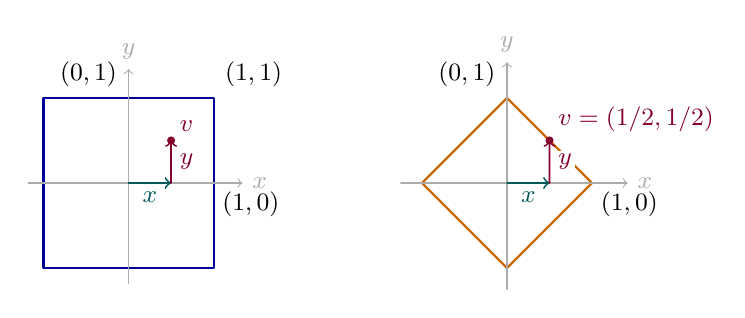
\begin{tikzpicture}[
  scale=1.08,
  font=\small,
  line cap=round,
  line join=round,
  axis/.style={gray!65, ->},
  maxball/.style={blue!60!black, thick},
  sumball/.style={orange!80!black, thick},
  xcomp/.style={teal!70!black, ->, line width=0.65pt},
  ycomp/.style={purple!70!black, ->, line width=0.65pt},
  pointlabel/.style={purple!70!black, fill=white, inner sep=1pt},
  metriclabel/.style={fill=white, inner sep=1pt}
]
  \begin{scope}
    \draw[maxball] (-1,-1) rectangle (1,1);
    \draw[axis] (-1.18,0) -- (1.34,0) node[right] {$x$};
    \draw[axis] (0,-1.18) -- (0,1.34) node[above] {$y$};
    \coordinate (vmax) at (0.5,0.5);
    \draw[xcomp] (0,0) -- (0.5,0);
    \draw[ycomp] (0.5,0) -- (vmax);
    \fill[purple!70!black] (vmax) circle (1.35pt);
    \node[pointlabel, above right=2pt] at (vmax) {$v$};
    \node[teal!70!black, below=2pt, metriclabel] at (0.25,0) {$x$};
    \node[purple!70!black, right=2pt, metriclabel] at (0.5,0.25) {$y$};
    \node[above left=3pt, metriclabel] at (0,1) {$(0,1)$};
    \node[above right=3pt, metriclabel] at (1,1) {$(1,1)$};
    \node[below right=2pt, metriclabel] at (1,0) {$(1,0)$};
  \end{scope}

  \begin{scope}[xshift=4.45cm]
    \draw[sumball] (0,1) -- (1,0) -- (0,-1) -- (-1,0) -- cycle;
    \draw[axis] (-1.25,0) -- (1.42,0) node[right] {$x$};
    \draw[axis] (0,-1.25) -- (0,1.42) node[above] {$y$};
    \coordinate (vsum) at (0.5,0.5);
    \draw[xcomp] (0,0) -- (0.5,0);
    \draw[ycomp] (0.5,0) -- (vsum);
    \fill[purple!70!black] (vsum) circle (1.35pt);
    \node[pointlabel, above right=2pt] at (vsum) {$v=(1/2,1/2)$};
    \node[teal!70!black, below=2pt, metriclabel] at (0.25,0) {$x$};
    \node[purple!70!black, right=2pt, metriclabel] at (0.5,0.25) {$y$};
    \node[above left=3pt, metriclabel] at (0,1) {$(0,1)$};
    \node[below right=2pt, metriclabel] at (1,0) {$(1,0)$};
  \end{scope}
\end{tikzpicture}

  \caption{Unit balls in $\R^2$: \textcolor{blue!60!black}{$\max\{\abs{x},\abs{y}\}<1$} and \textcolor{orange!80!black}{$\abs{x}+\abs{y}<1$}.}
  \label{fig:product-metric-unit-balls}
\end{figure}

\begin{proposition} \label{prop:balls-and-cells-convex} \hlt{Balls and Cells Are Convex}\\
Open balls, closed balls, and $k$-cells in $\R^k$ are convex.
\begin{proof}
Let $\mathbf{y},\mathbf{z}\in B_r(\mathbf{x})$ and $0<\lambda<1$.\\
Then $\norm{\lambda\mathbf{y}+(1-\lambda)\mathbf{z}-\mathbf{x}}_2 =\norm{\lambda(\mathbf{y}-\mathbf{x})+(1-\lambda)(\mathbf{z}-\mathbf{x})}_2 \leq \lambda\norm{\mathbf{y}-\mathbf{x}}_2+(1-\lambda)\norm{\mathbf{z}-\mathbf{x}}_2<r$.\\
The same proof with $\leq r$ gives closed balls. For a $k$-cell, each coordinate of $\lambda\mathbf{y}+(1-\lambda)\mathbf{z}$ lies between the corresponding coordinates of $\mathbf{y}$ and $\mathbf{z}$, hence remains in the same interval $[a_i,b_i]$.\\
\hlt{Structural Commentary}: Convexity is checked by following the line segment between two points.\\
\hlt{Key Insight}: Balls use the triangle inequality; cells use coordinate inequalities.
\end{proof}
\end{proposition}

\begin{definition} \label{def:product-metrics} \hlt{Product Metrics}\\
For metric spaces $(X,d_X)$ and $(Y,d_Y)$, and $p=(x,y)$, $p'=(x',y')$ in $X\times Y$, define
\begin{align}
d_E(p,p')&\defeq\sqrt{d_X(x,x')^2+d_Y(y,y')^2},\nonumber \\
d_{\max}(p,p')&\defeq\max\{d_X(x,x'),d_Y(y,y')\},\nonumber \\
d_{\mathrm{sum}}(p,p')&\defeq d_X(x,x')+d_Y(y,y') \nonumber
\end{align}
These are the Euclidean, maximum, and sum product metrics; the sum metric is often simplest for estimates.
\end{definition}

\begin{proposition} \label{prop:product-metric-comparison} \hlt{Comparing Product Metrics}\\
On $X\times Y$, $d_{\max}\leq d_E\leq d_{\mathrm{sum}}\leq2d_{\max}$. Hence the three product metrics have same convergent sequences.
\begin{proof}
Let $a=d_X(x,x')$ and $b=d_Y(y,y')$.\\
Then $\max\{a,b\}\leq\sqrt{a^2+b^2}\leq a+b\leq2\max\{a,b\}$; convergence follows by squeezing.\\
\hlt{Structural Commentary}: The three product metrics differ by controlled constants.\\
\hlt{Key Insight}: Equivalent metric estimates preserve convergence.
\end{proof}
\end{proposition}

\begin{proposition} \label{prop:bounded-compression-metric-same-open-sets} \hlt{Bounded Compression of a Metric}\\
If $(X,d)$ is a metric space, then $\rho(x,y)\defeq d(x,y)/(1+d(x,y))$ is a bounded metric on $X$, and $\tau_\rho=\tau_d$.
\begin{proof}
$0\leq\rho<1$, and definiteness and symmetry follow from $d$.\\
For $a,b\geq0$, $(a+b)/(1+a+b)\leq a/(1+a)+b/(1+b)$.\\
Since $t/(1+t)$ is increasing, $d(x,z)\leq d(x,y)+d(y,z)$ gives $\rho(x,z)\leq\rho(x,y)+\rho(y,z)$.\\
For balls, $B_d(x,\eta)\subseteq B_\rho(x,\eta)$ for $0<\eta<1$, and $B_\rho(x,\eta)\subseteq B_d(x,\eta/(1-\eta))$; hence $\tau_\rho=\tau_d$.\\
\hlt{Structural Commentary}: Compressing distances into $[0,1)$ changes boundedness but not local neighborhoods.\\
\hlt{Key Insight}: Topology depends on small-scale control, not on the large-scale size of distances.
\end{proof}
\end{proposition}

\begin{figure}[H]
  \centering
  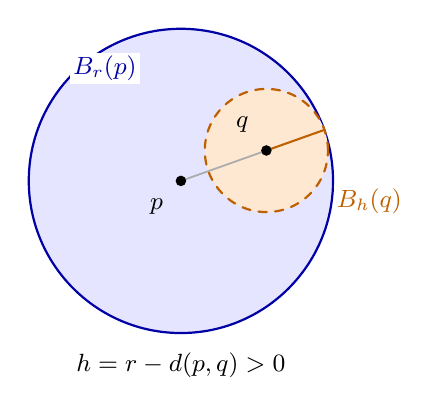
\begin{tikzpicture}[
  scale=0.92,
  every node/.style={font=\small},
  line cap=round,
  line join=round,
  outerball/.style={fill=blue!10, draw=blue!65!black, line width=0.8pt},
  innerball/.style={fill=orange!18, draw=orange!75!black, dashed, line width=0.8pt},
  guide/.style={gray!65, line width=0.65pt},
  gap/.style={orange!75!black, line width=0.75pt},
  point/.style={circle, fill=black, inner sep=1.35pt},
  labelbox/.style={fill=white, inner sep=1.2pt}
]
  \coordinate (p) at (0,0);
  \coordinate (q) at (1.18,0.42);
  \coordinate (b) at (1.979,0.704);

  \draw[outerball] (p) circle (2.10);
  \draw[innerball] (q) circle (0.85);

  \draw[guide] (p) -- (q);
  \draw[gap] (q) -- (b);

  \node[point,label={[label distance=2pt]below left:$p$}] at (p) {};
  \node[point,label={[label distance=2pt]above left:$q$}] at (q) {};
  \node[blue!65!black, labelbox] at (-1.05,1.55) {$B_r(p)$};
  \node[orange!75!black, labelbox, anchor=west] at (2.10,-0.28) {$B_h(q)$};

  \node[align=center, labelbox] at (0,-2.55) {$h=r-d(p,q)>0$};
\end{tikzpicture}

  \caption{Every point inside a metric ball has a smaller ball still contained in the original ball.}
  \label{fig:metric-ball-topology}
\end{figure}

\begin{definition} \label{def:metric-topology-core-definitions}\label{def:metric-topology-core-definitions-source-todo} \hlt{Metric Topology Terminology}\\
Let $X$ be a metric space, and let all points and sets below be understood as points of $X$ and subsets of $X$.
\begin{enumerate}[label=(\roman*)]
\setlength{\itemsep}{0pt}
\item A \hlt{neighborhood} of $p$ with radius $r>0$ is $B_r(p)\defeq\{q\in X:d(p,q)<r\}$.\\
The corresponding \hlt{closed ball} is $\overline{B}_r(p)\defeq\{q\in X:d(p,q)\leq r\}$, and the \hlt{sphere} of radius $r$ about $p$ is $\{q\in X:d(p,q)=r\}$.
\item A point $p$ is a \hlt{limit point} of $E$ if every neighborhood of $p$ contains a point $q\neq p$ with $q\in E$.
\item If $p\in E$ and $p$ is not a limit point of $E$, then $p$ is an \hlt{isolated point} of $E$.
\item A set $E$ is \hlt{closed} if every limit point of $E$ is a point of $E$.
\item A point $p$ is an \hlt{interior point} of $E$ if some neighborhood of $p$ is contained in $E$.
\item A set $E$ is \hlt{open} if every point of $E$ is an interior point of $E$.
\item The \hlt{complement} of $E$ is $E^c\defeq X\setminus E$.
\item A set $E$ is \hlt{dense} in $X$ if every point of $X$ is either a limit point of $E$, a point of $E$, or both.
\end{enumerate}
For $X=\R$, this gives $B_\varepsilon(a)=(a-\varepsilon,a+\varepsilon)$.\\
\hlt{Structural Commentary}: Openness and closedness are ambient notions, not opposites.
\end{definition}

\begin{example} \label{ex:open-closed-neither-and-both} \hlt{Open, Closed, Both, or Neither}\\
In $\R$, $\emptyset,\R$ are open and closed, while $[a,b)$, $a<b$, is neither. If $d$ is discrete on $X$, then $B_{1/2}(x)=\{x\}$ for all $x\in X$, so every $E\subseteq X$ and $E^c$ are open; hence every $E\subseteq X$ is closed.
\end{example}

\begin{theorem} \label{thm:every-neighborhood-open} \hlt{Every Neighborhood Is Open}\\
Every neighborhood in a metric space is an open set.
\begin{proof}
Let $E=B_r(p)$, and choose $q\in E$. Put $h\defeq r-d(p,q)>0$.\\
If $s\in B_h(q)$, then $d(p,s)\leq d(p,q)+d(q,s)<d(p,q)+h=r$.\\
Thus $B_h(q)\subseteq E$, so $q$ is an interior point of $E$. Since $q$ was arbitrary, $E$ is open.\\
\hlt{Structural Commentary}: Around any point inside a ball, the leftover distance to boundary gives a smaller ball.\\
\hlt{Key Insight}: The triangle inequality turns radius slack into openness.
\end{proof}
\end{theorem}

\begin{corollary} \label{cor:closed-balls-are-closed} \hlt{Closed Balls Are Closed}\\
For every $p\in X$ and $r>0$, the closed ball $\overline{B}_r(p)$ is closed.
\begin{proof}
Let $q\notin\overline{B}_r(p)$, so $d(p,q)>r$. Put $h\defeq(d(p,q)-r)/2$.\\
If $s\in B_h(q)$, then $d(p,s)\geq d(p,q)-d(q,s)>d(p,q)-h>r$, so $s\notin\overline{B}_r(p)$.\\
Hence the complement of $\overline{B}_r(p)$ is open, and $\overline{B}_r(p)$ is closed.\\
\hlt{Structural Commentary}: Outside a closed ball, positive distance remains to the boundary.\\
\hlt{Key Insight}: Reverse triangle estimates certify closedness.
\end{proof}
\end{corollary}

\begin{theorem} \label{thm:limit-point-neighborhoods-infinitely-many} \hlt{Limit Points Force Infinitely Many Nearby Points}\\
If $p$ is a limit point of $E$, then every neighborhood of $p$ contains infinitely many points of $E$.
\begin{proof}
Suppose some neighborhood $N$ of $p$ contains only finitely many points of $E$ distinct from $p$, say $q_1,\ldots,q_n$. If there are none, then $N$ itself contradicts that $p$ is a limit point. Otherwise put $\rho\defeq\min\limits_{1\leq m\leq n}d(p,q_m)>0$.\\
The neighborhood $B_\rho(p)$ contains no point $q\in E$ with $q\neq p$, contradicting the definition of limit point.\\
\hlt{Structural Commentary}: A finite list of nearby exceptions has a smallest positive distance from $p$.\\
\hlt{Key Insight}: Limit points cannot be witnessed by only finitely many neighboring points.
\end{proof}
\end{theorem}

\begin{corollary} \label{cor:finite-point-set-no-limit-points} \hlt{Finite Point Sets Have No Limit Points}\\
A finite point set in a metric space has no limit points.
\begin{proof}
Let $E\subseteq X$ be finite. If $p$ were a limit point of $E$, then by Theorem \ref{thm:limit-point-neighborhoods-infinitely-many}, every neighborhood of $p$ would contain infinitely many distinct points of $E$, impossible as $E$ is finite. Hence $E$ has no limit points.\\
\hlt{Structural Commentary}: This corollary is the finite obstruction to accumulation.\\
\hlt{Key Insight}: A limit point requires infinitely many nearby witnesses.
\end{proof}
\end{corollary}

\begin{theorem} \label{thm:open-iff-complement-closed} \hlt{Open Sets and Closed Complements}\\
A set $E$ is open if and only if its complement $E^c$ is closed.
\begin{proof}
\begin{enumerate}[label=\roman*.]
\setlength{\itemsep}{0pt}
\item[$(\Rightarrow)$] Suppose $E$ is open. If $x$ is a limit point of $E^c$ and $x\in E$, then some neighborhood $N$ of $x$ satisfies $N\subseteq E$, contradicting $N\cap(E^c\setminus\{x\})\neq\emptyset$. Hence $x\in E^c$, so $E^c$ is closed.
\item[$(\Leftarrow)$] Suppose $E^c$ is closed. If $x\in E$, then $x\notin E^c$, hence $x$ is not a limit point of $E^c$. Thus some neighborhood $N$ of $x$ has $N\cap E^c=\emptyset$, i.e. $N\subseteq E$. Hence $E$ is open.
\end{enumerate}
\hlt{Structural Commentary}: Openness of a set is equivalent to closure of the outside.\\
\hlt{Key Insight}: Interior points of $E$ cannot be limit points of $E^c$.
\end{proof}
\end{theorem}

\begin{corollary} \label{cor:closed-iff-complement-open} \hlt{Closed Sets and Open Complements}\\
A set $F$ is closed if and only if $F^c$ is open.
\begin{proof}
Apply Theorem \ref{thm:open-iff-complement-closed} with $E=F^c$. Then $F^c$ is open if and only if $(F^c)^c$ is closed. Since $(F^c)^c=F$, this is exactly the assertion that $F^c$ is open if and only if $F$ is closed.\\
\hlt{Structural Commentary}: This is the same open--closed duality after taking complements.\\
\hlt{Key Insight}: Closedness of $F$ is openness of the outside $F^c$.
\end{proof}
\end{corollary}

\begin{theorem} \label{thm:metric-open-closed-set-calculus}\label{prop:metric-topology-basic-calculus-source-todo} \hlt{Basic Topological Calculus}\\
In a metric space:
\begin{enumerate}[label=(\roman*)]
\setlength{\itemsep}{0pt}
\item any union of open sets is open;
\item any intersection of closed sets is closed;
\item any finite intersection of open sets is open;
\item any finite union of closed sets is closed.
\end{enumerate}
\begin{proof}
\begin{enumerate}[label=(\roman*)]
\setlength{\itemsep}{0pt}
\item Let $G\defeq\bigcup_\alpha G_\alpha$. If $x\in G$, then $x\in G_\alpha$ for some $\alpha$.\\
Since $G_\alpha$ is open, some neighborhood of $x$ lies in $G_\alpha\subseteq G$. Hence $G$ is open.
\item Let $F\defeq\bigcap_\alpha F_\alpha$. By Theorem \ref{thm:metric-de-morgan-laws}, $F^c=\bigcup\limits_\alpha F_\alpha^c$.\\
Each $F_\alpha^c$ is open by Corollary \ref{cor:closed-iff-complement-open}, so $F^c$ is open by (i). Hence $F$ is closed.
\item Let $H\defeq\bigcap\limits_{i=1}^nG_i$. If $x\in H$, let $r_i>0$, $B_{r_i}(x)\subseteq G_i$, $r\defeq\min_{1\leq i\leq n}r_i$. Then $B_r(x)\subseteq H$, so $H$ is open.
\item Let $F\defeq\bigcup_{i=1}^nF_i$. By Theorem \ref{thm:metric-de-morgan-laws}, $F^c=\bigcap\limits_{i=1}^nF_i^c$.\\
Each $F_i^c$ is open by Corollary \ref{cor:closed-iff-complement-open}, so $F^c$ is open by (iii). Hence $F$ is closed.
\end{enumerate}
\hlt{Structural Commentary}: Arbitrary unions are easy for open sets; finite intersections require a minimum radius.\\
\hlt{Key Insight}: The finite minimum is the reason infinite intersections of open sets need not be open.
\end{proof}
\end{theorem}

\begin{definition} \label{def:metric-closure} \hlt{Closure}\\
If $E\subseteq X$ and $E^{\operatorname{acc}}$ denotes the set of all limit points of $E$ in $X$, then the \hlt{closure} of $E$ is $\overline{E}\defeq E\cup E^{\operatorname{acc}}$.
\end{definition}

\begin{theorem} \label{thm:closure-smallest-closed-containing-set} \hlt{Closure Is the Smallest Closed Superset}\\
If $X$ is a metric space and $E\subseteq X$, then:
\begin{enumerate}[label=(\roman*)]
\setlength{\itemsep}{0pt}
\item $\overline{E}$ is closed;
\item $\overline{E}=E$ if and only if $E$ is closed;
\item $\overline{E}\subseteq F$ for every closed set $F\subseteq X$ such that $E\subseteq F$.
\end{enumerate}
Thus $\overline{E}$ is the smallest closed subset of $X$ that contains $E$.
\begin{proof}
\begin{enumerate}[label=(\roman*)]
\setlength{\itemsep}{0pt}
\item Let $p\notin\overline{E}$. Then $p\notin E$ and $p$ is not a limit point of $E$, so $B_r(p)\cap E=\emptyset$ for some $r>0$. If $q\in B_r(p)$, then $q\notin E$ and $B_{r-d(p,q)}(q)\subseteq B_r(p)$, so $q\notin E^{\operatorname{acc}}$.\\
Hence $B_r(p)\subseteq(\overline{E})^c$, and $\overline{E}$ is closed by Corollary \ref{cor:closed-iff-complement-open}.
\item If $\overline{E}=E$, then $E$ is closed by (i). Conversely, if $E$ is closed, then $E^{\operatorname{acc}}\subseteq E$, so $\overline{E}=E\cup E^{\operatorname{acc}}=E$.
\item If $F$ is closed and $E\subseteq F$, then $E^{\operatorname{acc}}\subseteq F^{\operatorname{acc}}\subseteq F$. Thus $\overline{E}=E\cup E^{\operatorname{acc}}\subseteq F$.
\end{enumerate}
\hlt{Structural Commentary}: Closure adds exactly the limit points forced by $E$.\\
\hlt{Key Insight}: Closed supersets must contain all limit points, so they must contain $\overline{E}$.
\end{proof}
\end{theorem}

\begin{figure}[H]
  \centering
  % Source guide: Roman, Advanced Linear Algebra, Ch. 12, Figure 12.1.
% Redrawn as the inner-ball containment used in closure and limit-point proofs.
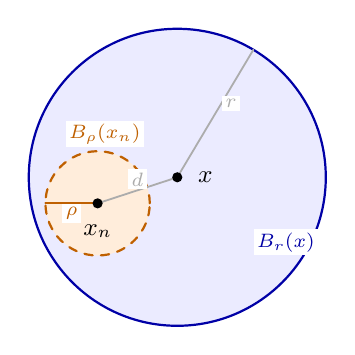
\begin{tikzpicture}[
  scale=0.92,
  every node/.style={font=\small},
  line cap=round,
  line join=round,
  outerball/.style={draw=blue!65!black, fill=blue!8, line width=0.8pt},
  innerball/.style={draw=orange!75!black, fill=orange!14, dashed, line width=0.8pt},
  guide/.style={gray!65, line width=0.65pt},
  gap/.style={orange!75!black, line width=0.7pt},
  point/.style={circle, fill=black, inner sep=1.3pt},
  note/.style={font=\scriptsize, fill=white, inner sep=1.2pt}
]
  \coordinate (x) at (0.65,0.18);
  \coordinate (xn) at (-0.45,-0.18);
  \coordinate (outerpt) at (1.70,1.94);
  \coordinate (innerpt) at (-1.17,-0.18);

  \draw[outerball] (x) circle (2.05);
  \draw[innerball] (xn) circle (0.72);

  \draw[guide] (x) -- node[note, pos=0.58, right] {$r$} (outerpt);
  \draw[guide] (x) -- node[note, midway, above] {$d$} (xn);
  \draw[gap] (xn) -- node[note, midway, below] {$\rho$} (innerpt);

  \node[point,label={[label distance=2pt]right:$x$}] at (x) {};
  \node[point,label={[label distance=2pt]below:$x_n$}] at (xn) {};

  \node[note, text=blue!65!black] at (2.15,-0.72) {$B_r(x)$};
  \node[note, text=orange!75!black] at (-0.35,0.78) {$B_\rho(x_n)$};
\end{tikzpicture}

  \caption{If $d=d(x,x_n)<r$, then any $0<\rho<r-d$ gives
  $B_\rho(x_n)\subseteq B_r(x)$.}
  \label{fig:limit-point-closure-inner-ball}
\end{figure}

\begin{definition} \label{def:interior-closure-boundary}\label{def:adherent-points-and-closure}\label{def:set-distance-in-metric-space} \hlt{Interior, Boundary, Adherence, and Distance}\\
Let $(X,d)$ be a metric space and $E,F\subseteq X$.
\begin{enumerate}[label=(\roman*)]
\setlength{\itemsep}{0pt}
\item $E^\circ\defeq\{p\in E:\exists r>0,\ B_r(p)\subseteq E\}$ is the \hlt{interior}
\item $\operatorname{ext}(E)\defeq(E^c)^\circ=\{p\in X:\exists r>0,\ B_r(p)\cap E=\emptyset\}$ is the \hlt{exterior}.
\item $\operatorname{bd}(E)\defeq\overline{E}\setminus E^\circ=\{p\in X:\forall r>0,\ B_r(p)\cap E\ne\emptyset,\ B_r(p)\cap E^c\ne\emptyset\}$ is the \hlt{boundary}.
\item $p\in X$ is \hlt{adherent} to $E$ iff $\forall r>0,\ B_r(p)\cap E\ne\emptyset$, equivalently $p\in\overline{E}$.
\item For $p\in X$, nonempty $E,F$, $\operatorname{dist}(p,E)\defeq\inf\{d(p,q):q\in E\}$' $\operatorname{dist}(E,F)\defeq\inf\{d(p,q):p\in E,\ q\in F\}$.
\end{enumerate}
\end{definition}

\begin{figure}[H]
  \centering
  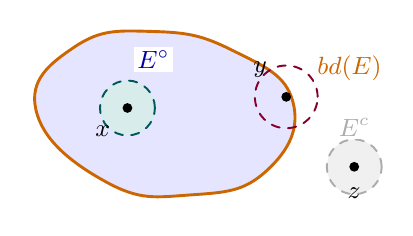
\begin{tikzpicture}[
  scale=0.83,
  every node/.style={font=\small},
  line cap=round,
  line join=round,
  set/.style={fill=blue!10, draw=orange!80!black, line width=1.05pt},
  ballin/.style={fill=teal!15, draw=teal!70!black, dashed, line width=0.7pt},
  ballbd/.style={draw=purple!70!black, dashed, line width=0.7pt},
  ballex/.style={fill=gray!12, draw=gray!65, dashed, line width=0.7pt},
  point/.style={circle, fill=black, inner sep=1.25pt},
  note/.style={fill=white, inner sep=1.1pt}
]
  \draw[set]
    plot[smooth cycle, tension=0.8] coordinates {
      (-2.15,0.15) (-1.55,1.12) (-0.35,1.35) (0.88,1.05)
      (1.78,0.28) (1.38,-0.78) (0.22,-1.15) (-1.08,-0.95)
    };

  \coordinate (i) at (-0.75,0.18);
  \coordinate (b) at (1.68,0.35);
  \coordinate (e) at (2.72,-0.72);

  \draw[ballin] (i) circle (0.42);
  \draw[ballbd] (b) circle (0.48);
  \draw[ballex] (e) circle (0.42);

  \node[point,label={[label distance=2pt]below left:$x$}] at (i) {};
  \node[point,label={[label distance=3pt]above left:$y$}] at (b) {};
  \node[point,label={[label distance=2pt]below:$z$}] at (e) {};

  \node[blue!65!black, note] at (-0.35,0.92) {$E^\circ$};
  \node[orange!80!black, note, anchor=west] at (2.10,0.78) {$\operatorname{bd}(E)$};
  \node[gray!65, note] at (2.72,-0.12) {$E^c$};
\end{tikzpicture}

  \caption{Interior, exterior, and boundary points are distinguished by how small balls meet $E$ and $E^c$.}
  \label{fig:metric-ball-closure-boundary}
\end{figure}

\begin{proposition} \label{prop:set-distance-closure-criterion} \hlt{Distance-to-Set Closure Criterion}\\
Let $\emptyset\ne E\subseteq X$. For $p\in X$, $p\in\overline{E}\Longleftrightarrow \operatorname{dist}(p,E)=0$.
\begin{proof}
\begin{enumerate}[label=\roman*.]
\setlength{\itemsep}{0pt}
\item[$(\Rightarrow)$] If $p\in\overline{E}$, then $\forall\varepsilon>0$, $B_\varepsilon(p)\cap E\ne\emptyset$; choose $q_\varepsilon\in E$ with $d(p,q_\varepsilon)<\varepsilon$.\\
Thus $0\leq\operatorname{dist}(p,E)\leq\varepsilon$ for all $\varepsilon>0$, so $\operatorname{dist}(p,E)=0$.
\item[$(\Leftarrow)$] If $\operatorname{dist}(p,E)=0$, then $\forall r>0$, $\exists q\in E$ with $d(p,q)<r$.\\
Hence $B_r(p)\cap E\ne\emptyset$ for all $r>0$, so $p$ is adherent to $E$, equivalently $p\in\overline{E}$.
\end{enumerate}
\hlt{Structural Commentary}: Closure can be detected by vanishing distance to the set.\\
\hlt{Key Insight}: The infimum packages all small-ball tests into one number.
\end{proof}
\end{proposition}

\begin{remark} \label{rem:set-distance-is-not-subset-metric} \hlt{Set Distance Is Not a Metric on Subsets}\\
The function $\operatorname{dist}(E,F)$ is useful, but it is not a metric on nonempty subsets.\\
In $\R$, for example, $\operatorname{dist}((0,1),(1,2))=0$ although the sets are distinct and disjoint.
\end{remark}

\begin{figure}[H]
  \centering
  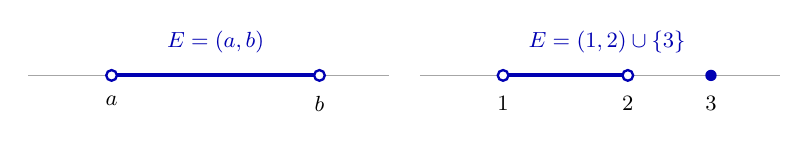
\begin{tikzpicture}[
  scale=0.88,
  transform shape,
  every node/.style={font=\small},
  axis/.style={gray!70, line width=0.55pt},
  setbar/.style={blue!70!black, line width=1.45pt, line cap=round},
  openpt/.style={circle, draw=blue!70!black, fill=white, line width=0.85pt, inner sep=1.55pt},
  point/.style={circle, fill=blue!70!black, inner sep=1.65pt},
  note/.style={fill=white, inner sep=1.2pt}
]
  \begin{scope}
    \draw[axis] (-0.25,0) -- (4.95,0);
    \draw[setbar] (0.95,0) -- (3.95,0);
    \node[openpt] at (0.95,0) {};
    \node[openpt] at (3.95,0) {};

    \node[below=5pt] at (0.95,0) {$a$};
    \node[below=5pt] at (3.95,0) {$b$};
    \node[above=8pt, blue!70!black, note] at (2.45,0) {$E=(a,b)$};
  \end{scope}

  \begin{scope}[xshift=5.65cm]
    \draw[axis] (-0.25,0) -- (4.95,0);
    \draw[setbar] (0.95,0) -- (2.75,0);
    \node[openpt] at (0.95,0) {};
    \node[openpt] at (2.75,0) {};
    \node[point] at (3.95,0) {};

    \node[below=5pt] at (0.95,0) {$1$};
    \node[below=5pt] at (2.75,0) {$2$};
    \node[below=5pt] at (3.95,0) {$3$};
    \node[above=8pt, blue!70!black, note] at (2.45,0) {$E=(1,2)\cup\{3\}$};
  \end{scope}
\end{tikzpicture}

  \caption{Adherent endpoints need not lie in $E$; isolated points are adherent but not limit points.}
  \label{fig:adherent-limit-isolated-points}
\end{figure}

\begin{definition} \label{def:bounded-and-perfect-metric-sets}\label{rem:boundedness-and-intrinsic-metric-properties}\label{per:metric-sequences-as-topological-tests}\label{def:sequence-convergence-metric}\label{def:sequences-core-definitions-source-todo}\label{def:sequence-range-and-boundedness}\label{def:eventually-and-frequently-in-a-set} \hlt{Bounded Sets and Metric Sequences}\\
Let $(X,d)$ be a metric space, $E\subseteq X$, and $(p_n)$ a sequence in $X$.
\begin{enumerate}[label=(\roman*)]
\setlength{\itemsep}{0pt}
\item $E$ is \hlt{bounded} iff $\exists q\in X,\exists M>0$ such that $E\subseteq B_M(q)$
\item $E$ is \hlt{perfect} iff $E$ is closed and every $p\in E$ is a limit point of $E$.
\item $(p_n)$ \hlt{converges} to $p\in X$ iff $\forall\varepsilon>0,\exists N\in\N$ such that $n\geq N\Longrightarrow d(p_n,p)<\varepsilon$; write $p_n\to p$ or $\lim\limits_{n\to\infty}p_n=p$.\\
If no such $p$ exists, $(p_n)$ \hlt{diverges}.
\item The \hlt{range} of $(p_n)$ is $\operatorname{ran}(p_n)\defeq\{p_n:n\in\N\}$; $(p_n)$ is \hlt{bounded} iff $\operatorname{ran}(p_n)$ is bounded.
\item $(p_n)$ is \hlt{eventually in $E$} iff $\exists N\in\N$ such that $n\geq N\Longrightarrow p_n\in E$
\item $(p_n)$ is \hlt{frequently in $E$} iff $\forall N\in\N,\exists n\geq N$ such that $p_n\in E$.
\end{enumerate}
\hlt{Structural Commentary}: Boundedness, compactness, and completeness are intrinsic to restricted metrics; openness and closedness are ambient.\\
\hlt{Key Insight}: Convergence is tail control; frequent membership is arbitrarily late recurrence.
\end{definition}

\begin{proposition} \label{prop:sequence-limit-points-subsequential-limits} \hlt{Limit Points Are Subsequence Limits}\\
For $(p_n)\subseteq X$ and $p\in X$, the following are equivalent:
\begin{enumerate}[label=(\roman*)]
\setlength{\itemsep}{0pt}
\item $\forall r>0,\forall N\in\N,\exists n\geq N$ such that $p_n\in B_r(p)$.
\item $\exists n_1<n_2<\cdots$ such that $p_{n_k}\to p$.
\end{enumerate}
\begin{proof}
\begin{enumerate}[label=\roman*.]
\setlength{\itemsep}{0pt}
\item[$(i)$]$\Rightarrow(ii)$ Set $n_0=0$. By (i), recurse $n_k>n_{k-1}$ with $p_{n_k}\in B_{1/k}(p)$; then $d(p_{n_k},p)<1/k$, so $p_{n_k}\to p$.
\item[$(ii)$]$\Rightarrow(i)$ If $p_{n_k}\to p$, then for any $r>0$ and $N\in\N$, choose $k$ with $n_k\geq N$ and $d(p_{n_k},p)<r$.\\
Thus $p_{n_k}\in B_r(p)$, so (i) holds.
\end{enumerate}
\hlt{Structural Commentary}: Frequent visits are exactly enough to extract a convergent subsequence.\\
\hlt{Key Insight}: Limits require all sufficiently late terms; limit points require arbitrarily late witnesses.
\end{proof}
\end{proposition}

\begin{theorem} \label{thm:metric-sequence-basic-properties} \hlt{Basic Properties of Metric Convergence}\\
Let $X$ be a metric space and $(p_n)\subseteq X$.
\begin{enumerate}[label=(\roman*)]
\setlength{\itemsep}{0pt}
\item $p_n\to p\Longleftrightarrow\forall r>0,\exists N\in\N$ such that $n\geq N\Longrightarrow p_n\in B_r(p)$.
\item If $p_n\to p$ and $p_n\to p'$, then $p=p'$.
\item If $E\subseteq X$ and $p\in E^{\operatorname{acc}}$, then $\exists(q_n)\subseteq E\setminus\{p\}$ such that $q_n\to p$.
\end{enumerate}
\begin{proof}
\begin{enumerate}[label=(\roman*).]
\setlength{\itemsep}{0pt}
\item[$(i)$]($\Rightarrow$) If $p_n\to p$ and $r>0$, take $\varepsilon=r$ in the definition.
\item[$(i)$]($\Leftarrow$) If the ball condition holds, then for every $\varepsilon>0$ take $r=\varepsilon$, giving $d(p_n,p)<\varepsilon$ eventually.
\item[$(ii)$] Given $\varepsilon>0$, choose $N,N'$ with $n\geq N\Longrightarrow d(p_n,p)<\varepsilon/2$ and $n\geq N'\Longrightarrow d(p_n,p')<\varepsilon/2$.\\
If $n\geq\max\{N,N'\}$, then $d(p,p')\leq d(p,p_n)+d(p_n,p')<\varepsilon$, so $d(p,p')=0$.
\item[$(iii)$] Since $p\in E^{\operatorname{acc}}$, for each $n\in\N$ choose $q_n\in E\setminus\{p\}$ with $d(q_n,p)<1/n$. Then $q_n\to p$.
\end{enumerate}
\hlt{Structural Commentary}: Eventual containment gives convergence; triangle inequality gives uniqueness.\\
\hlt{Key Insight}: A limit point can always be approached by a sequence of points from the set.
\end{proof}
\end{theorem}

\begin{corollary} \label{cor:metric-convergent-subsequences} \hlt{Subsequences Preserve Metric Limits}\\
If $p_n\to p$ in a metric space, then every subsequence $(p_{n_k})$ also converges to $p$.
\begin{proof}
Given $\varepsilon>0$, choose $N$ such that $n\geq N$ implies $d(p_n,p)<\varepsilon$.\\
Since $n_k\to\infty$, all sufficiently large $k$ satisfy $n_k\geq N$, hence $d(p_{n_k},p)<\varepsilon$.\\
\hlt{Structural Commentary}: A subsequence is only a delayed tail of the same sequence.\\
\hlt{Key Insight}: Eventual estimates survive deleting terms.
\end{proof}
\end{corollary}

\begin{proposition} \label{prop:discrete-metric-convergence-eventually-constant} \hlt{Discrete-Metric Convergence}\\
Let $X$ carry the discrete metric $d(x,y)=0$ if $x=y$ and $d(x,y)=1$ if $x\neq y$.\\
For $(p_n)\subset X$ and $p\in X$, $p_n\to p$ if and only if $\exists N\in\N$ such that $n\geq N\Longrightarrow p_n=p$.
\begin{proof}
\begin{enumerate}[label=\roman*.]
\setlength{\itemsep}{0pt}
\item[$(\Rightarrow)$] Suppose $p_n\to p$. For $\varepsilon=1/2$, choose $N\in\N$ such that $n\geq N\Longrightarrow d(p_n,p)<1/2$.\\
Since $d$ takes only the values $0,1$, $d(p_n,p)=0$, hence $p_n=p$ for all $n\geq N$.
\item[$(\Leftarrow)$] Suppose $\exists N\in\N$ s.t. $n\geq N\Longrightarrow p_n=p$. Then $\forall \varepsilon>0$, $n\geq N$ gives $d(p_n,p)=0<\varepsilon$, so $p_n\to p$.
\end{enumerate}
\hlt{Structural Commentary}: The discrete metric has no room for distinct points to approach one another.\\
\hlt{Key Insight}: In the discrete metric, $d(x,y)<1\Longleftrightarrow x=y$.
\end{proof}
\end{proposition}

\begin{proposition} \label{prop:sequential-closure-criterion} \hlt{Sequential Closure Criterion}\\
Let $E\subseteq X$, where $X$ is a metric space, and let $p\in X$. Then $p\in\overline{E}$ $\Longleftrightarrow$ $\exists (p_n)_{n\geq1}$ with $p_n\in E\ \forall n$, $p_n\to p$.
\begin{proof}
\begin{enumerate}[label=\roman*.]
\setlength{\itemsep}{0pt}
\item[$(\Rightarrow)$] If $p\in\overline{E}$, choose $p_n\in E\cap B_{1/n}(p)$ for $n\geq1$ by Principle \ref{princ:axiom-of-choice-analysis}. Then $d(p_n,p)<1/n$, so $p_n\to p$.
\item[$(\Leftarrow)$] If $p_n\in E$ and $p_n\to p$, then every ball $B_r(p)$ contains some $p_n$.\\
Thus $p$ is adherent to $E$ by Definition \ref{def:adherent-points-and-closure}, so $p\in\overline{E}$.
\end{enumerate}
\hlt{Structural Commentary}: Closure can be read either by neighborhoods or by sequences.\\
\hlt{Key Insight}: Adherence supplies one witness at every scale.
\end{proof}
\end{proposition}

\begin{theorem} \label{thm:closed-sets-and-limit-points-via-sequences} \hlt{Closed Sets and Limit Points via Sequences}\\
Let $X$ be a metric space and $E\subseteq X$.
\begin{enumerate}[label=(\roman*)]
\setlength{\itemsep}{0pt}
\item $p\in E^{\operatorname{acc}}\Longleftrightarrow\exists(p_n)\subseteq E\setminus\{p\}$ such that $p_n\to p$.
\item $E$ is closed $\Longleftrightarrow$ every $(p_n)\subseteq E$ with $p_n\to p\in X$ satisfies $p\in E$.
\end{enumerate}
\begin{proof}
\begin{enumerate}[label=(\roman*).]
\setlength{\itemsep}{0pt}
\item[$(i)$]($\Rightarrow$) If $p\in E^{\operatorname{acc}}$, choose $p_n\in(E\setminus\{p\})\cap B_{1/n}(p)$ for each $n$. Then $d(p_n,p)<1/n$, so $p_n\to p$.
\item[$(i)$]($\Leftarrow$) If $(p_n)\subseteq E\setminus\{p\}$ and $p_n\to p$, then every $B_r(p)$ contains some $p_n\ne p$. Hence $p\in E^{\operatorname{acc}}$.
\item[$(ii)$]($\Rightarrow$) If $E$ is closed, $(p_n)\subseteq E$, and $p_n\to p$, then Proposition \ref{prop:sequential-closure-criterion} gives $p\in\overline{E}=E$.
\item[$(ii)$]($\Leftarrow$) If every convergent sequence in $E$ has limit in $E$, then Proposition \ref{prop:sequential-closure-criterion} gives $\overline{E}\subseteq E$. QED.
\end{enumerate}
\hlt{Structural Commentary}: In metric spaces, closedness can be tested by sequences.\\
\hlt{Key Insight}: Balls at radii $1/n$ convert local information into a sequence.
\end{proof}
\end{theorem}

\begin{proposition} \label{prop:dense-closure-criterion} \hlt{Density and Closure}\\
Let $X$ be a metric space and let $E\subseteq X$. Then $E$ is dense in $X$ if and only if $\overline{E}=X$.
\begin{proof}
\begin{enumerate}[label=\roman*.]
\setlength{\itemsep}{0pt}
\item[$(\Rightarrow)$] Suppose $E$ is dense in $X$. Let $p\in X$. By Definition \ref{def:metric-topology-core-definitions}, $p$ is either a point of $E$ or a limit point of $E$. Hence $p\in E\cup E^{\operatorname{acc}}=\overline{E}$ by Definition \ref{def:metric-closure}. Thus $X\subseteq\overline{E}$. Since $\overline{E}\subseteq X$, $\overline{E}=X$.
\item[$(\Leftarrow)$] Suppose $\overline{E}=X$. Let $p\in X$. Then $p\in\overline{E}=E\cup E^{\operatorname{acc}}$, so $p$ is either a point of $E$ or a limit point of $E$. Therefore $E$ is dense in $X$ by Definition \ref{def:metric-topology-core-definitions}.
\end{enumerate}
\hlt{Structural Commentary}: Density says every point is already in $E$ or is forced by nearby points of $E$.\\
\hlt{Key Insight}: The closure packages exactly those two possibilities.
\end{proof}
\end{proposition}

\begin{proposition} \label{prop:dense-closure-and-interval-test} \hlt{Real-Line Density Interval Test}\\
Let $E\subseteq\R$. Then $E$ is dense in $\R$ if and only if every nonempty open interval $(a,b)$ satisfies $(a,b)\cap E\neq\emptyset$.
\begin{proof}
\begin{enumerate}[label=\roman*.]
\setlength{\itemsep}{0pt}
\item[$(\Rightarrow)$] Let $(a,b)\ne\emptyset$ and choose $p\in(a,b)$, $r\defeq\frac12\min\{p-a,b-p\}$. If $p\in E$, done. If $p\notin E$, density gives $p\in E^{\operatorname{acc}}$, so choose $q\in(E\setminus\{p\})\cap B_r(p)$. Since $B_r(p)\subseteq(a,b)$, $q\in(a,b)\cap E$.
\item[$(\Leftarrow)$] Suppose $(a,b)\cap E\ne\emptyset$ for every nonempty open interval $(a,b)$. For $p\in\R$, either $p\in E$, or $p\notin E$ and $\forall\varepsilon>0$, choose $q\in(p-\varepsilon,p+\varepsilon)\cap E$. Then $q\ne p$ and $q\in B_\varepsilon(p)$, so $p\in E^{\operatorname{acc}}$. Hence $\R=E\cup E^{\operatorname{acc}}=\overline{E}$, so $E$ is dense in $\R$.
\end{enumerate}
\hlt{Structural Commentary}: On $\R$, balls and open intervals test the same local condition.\\
\hlt{Key Insight}: Density means no interval can avoid the set.
\end{proof}
\end{proposition}

\begin{definition} \label{def:separable-metric-space} \hlt{Separable Metric Space}\\
A metric space $X$ is \hlt{separable} if it contains a countable dense subset.
\end{definition}

\begin{example} \label{ex:separable-and-nonseparable-metric-spaces} \hlt{Separable and Nonseparable Metric Spaces}
\begin{enumerate}[label=(\roman*)]
\setlength{\itemsep}{0pt}
\item $\R$ is separable: $\Q$ is countable and dense. Hence $\R^k$ is separable via $\Q^k$, and $\C^k$ via $\C^k\simeq\R^{2k}$.
\item If $X$ is discrete, then $X$ is separable $\Longleftrightarrow X$ is countable,\\
since $B_{1/2}(x)=\{x\}$ forces every dense $D\subseteq X$ to contain $x$.
\item $\ell^\infty(\F)$ is not separable. The set $\{0,1\}^{\N}$ is uncountable, and $s\ne t$ gives $d_\infty(s,t)=1$; the balls $B_{1/3}(s)$ are pairwise disjoint, so no countable dense set can meet all of them.
\item For $1\leq p<\infty$, $\ell^p(\F)$ is separable. Let $D$ be the countable set of finite-support sequences with rational coordinates, using rational real and imaginary parts if $\F=\C$.\\
For $x\in\ell^p$ and $\varepsilon>0$, choose $N$ with $\sum_{n>N}\abs{x_n}^p<(\varepsilon/2)^p$, then choose $y\in D$ with support in $\{1,\ldots,N\}$ and $\sum_{n=1}^N\abs{x_n-y_n}^p<(\varepsilon/2)^p$. Thus $\norm{x-y}_p<\varepsilon$.
\end{enumerate}
\hlt{Structural Commentary}: Separability is the existence of a countable set meeting every nonempty open ball.\\
\hlt{Key Insight}: Finite rational data are dense in $\ell^p$, while $\ell^\infty$ contains an uncountable $1$-separated set.
\end{example}

\begin{theorem} \label{thm:supremum-belongs-to-closure} \hlt{Suprema Belong to Closures}\\
Let $\emptyset\ne E\subseteq\R$ be bounded above and $y\defeq\sup E$. Then $y\in\overline{E}$; if $E$ is closed, then $y\in E$.
\begin{proof}
If $y\in E$, then $y\in\overline{E}$. If $y\notin E$, then $\forall h>0$, $y-h$ is not an upper bound; choose $x_h\in E$ with $y-h<x_h\leq y$. Thus $x_h\ne y$, $\abs{x_h-y}<h$, and $B_h(y)\cap(E\setminus\{y\})\ne\emptyset$, so $y\in E^{\operatorname{acc}}\subseteq\overline{E}$.\\
If $E$ is closed, $\overline{E}=E$ by Theorem \ref{thm:closure-smallest-closed-containing-set}(ii).\\
\hlt{Structural Commentary}: LUB gives points of $E$ arbitrarily close below $\sup E$.\\
\hlt{Key Insight}: A supremum is either attained or approached.
\end{proof}
\end{theorem}

\begin{definition} \label{def:relative-open-subset} \hlt{Relative Openness}\\
Suppose $E\subseteq Y\subseteq X$, where $X$ is a metric space. The set $E$ is \hlt{open relative to $Y$} if for each $p\in E$ there is an $r>0$ such that $q\in E$ whenever $q\in Y$ and $d(p,q)<r$.
\end{definition}

\begin{theorem} \label{thm:relative-open-intersection-with-open-set} \hlt{Relative Opens Are Intersections}\\
Suppose $Y\subseteq X$. A subset $E$ of $Y$ is open relative to $Y$ if and only if $E=Y\cap G$ for some open subset $G$ of $X$.
\begin{proof}
\begin{enumerate}[label=\roman*.]
\setlength{\itemsep}{0pt}
\item[$(\Rightarrow)$] For each $p\in E$, choose $r_p>0$ with $B_{r_p}(p)\cap Y\subseteq E$, and set $G\defeq\bigcup\limits_{p\in E}B_{r_p}(p)$. Then $G$ is open in $X$, and $E\subseteq G\cap Y$. If $q\in G\cap Y$, then $q\in B_{r_p}(p)\cap Y$ for some $p\in E$, so $q\in E$. Thus $E=G\cap Y$.
\item[$(\Leftarrow)$] If $E=G\cap Y$ with $G$ open in $X$, then for each $p\in E$ choose $r>0$ with $B_r(p)\subseteq G$.\\
Hence $B_r(p)\cap Y\subseteq G\cap Y=E$, so $E$ is open relative to $Y$.
\end{enumerate}
\hlt{Structural Commentary}: Relative openness is ordinary openness viewed through the ambient subset $Y$.\\
\hlt{Key Insight}: Intersect open sets in $X$ with $Y$ to get exactly the open sets of $Y$.
\end{proof}
\end{theorem}

\begin{example} \label{ex:relative-topology-ambient-examples} \hlt{Relative Topology Depends on the Ambient Space}\\
Let $X=\{(x,0):x\in\R\}\subseteq\R^2$ with the metric inherited from $\R^2$. The set $E=\{(x,0):-1<x<1\}$ is not open as a subset of $\R^2$, but it is open relative to $X$, since $E=X\cap\bigl((-1,1)\times(-1,1)\bigr)$.\\
Likewise, $[0,1)$ is not closed in $\R$, but it is closed relative to $(-1,1)$ because $[0,1)=(-1,1)\cap[0,\infty)$.
\end{example}

\begin{method} \label{meth:metric-topology-proof-patterns}\label{meth:metric-topology-proof-patterns-source-todo} \hlt{Metric Proof Patterns}
\begin{enumerate}[label=(\roman*)]
\setlength{\itemsep}{0pt}
\item To prove $G$ is open, fix $x\in G$ and find $r>0$ with $B_r(x)\subseteq G$.
\item To prove $F$ is closed, show $F^{\operatorname{acc}}\subseteq F$, or equivalently show $F^c$ is open.
\item To prove $C=\overline{E}$, show $E\subseteq C$, $C$ is closed, and $C\subseteq F$ for every closed $F\supseteq E$.
\item To prove $p\in\overline{E}$, show $\operatorname{dist}(p,E)=0$, or build a sequence in $E$ converging to $p$.
\end{enumerate}
\end{method}
